\section{\Large PROBLEM SET 8}

\subsection{Problem 1 - The time update should be complete and verified at this stage. We need to include the incoming measurements. Search in literature or derive, define, and code a sensitivity matrix H which provides your state at step k+1 from your measurement vector at step k+1 (i.e., at the same current time, propagation has already been done).}

The sensitivity matrix is defined in Equation \ref{eq:general_sens_matrix} as being the Jacobian of the measurement model, $\vec{h}$, taken with respect to the state variables.

\begin{equation} \label{eq:general_sens_matrix}
    \boldsymbol{H} = \frac{\partial \vec{h}}{\partial \vec{x}}
\end{equation}

If the measurement model yields $N$ unit vectors of known direction in the inertial frame (i.e. star direction, sun direction, etc.) represented by vectors, $\vec{v}_i$, then it follows the form shown in Equation \ref{eq:attitude_meas_model}.

\begin{equation} \label{eq:attitude_meas_model}
    \vec{h}_{\alpha} = \begin{bmatrix}
        \boldsymbol{R}_{t+1 \vert t} \vec{v}_1 \\
        \boldsymbol{R}_{t+1 \vert t} \vec{v}_2 \\
        \vdots \\
        \boldsymbol{R}_{t+1 \vert t} \vec{v}_N
    \end{bmatrix} = \begin{bmatrix}
        \vec{h}_1 \\
        \vec{h}_2 \\
        \vdots \\
        \vec{h}_N
    \end{bmatrix}
\end{equation}

Therefore, the sensitivity matrix that corresponds to this measurement type is defined in Equation \ref{eq:attitude_sens_matrix}.

\begin{equation} \label{eq:attitude_sens_matrix}
    \boldsymbol{H}_{\alpha} = \begin{bmatrix}
        \boldsymbol{ \left[ h_1 \times \right] } & \boldsymbol{ \left[ h_2 \times \right] } & \dots & \boldsymbol{ \left[ h_N \times \right] }
    \end{bmatrix}^T
\end{equation}

In the state space that has been chosen for this Kalman Filter, however, there is also a component of the measurement and the component of the state that describe the angular velocity of the spacecraft about its principal axes. Tor this component of the measurement and state vector, the sensitivity matrix is simply identity, which is seen in Equations \ref{eq:vel_meas_model} and \ref{eq:vel_sens_matrix}.

\begin{equation} \label{eq:vel_meas_model}
    \vec{h}_{\omega} = \begin{bmatrix}
        \omega_x \\
        \omega_y \\
        \omega_z
    \end{bmatrix}
\end{equation}

\begin{equation} \label{eq:vel_sens_matrix}
    \boldsymbol{H}_{\omega} = \boldsymbol{I}
\end{equation}

Now constructing a block sensitivity matrix to span the full measurement model and state space, the full sensitivity matrix is shown in Equation \ref{eq:full_sens_matrix}.

\begin{equation} \label{eq:full_sens_matrix}
    \boldsymbol{H} = \begin{bmatrix}
        \boldsymbol{H}_{\alpha} & \boldsymbol{0} \\
        \boldsymbol{0} & \boldsymbol{H}_{\omega}
    \end{bmatrix} = \begin{bmatrix}
        \begin{bmatrix}
        \boldsymbol{ \left[ h_1 \times \right] } & \boldsymbol{ \left[ h_2 \times \right] } & \dots & \boldsymbol{ \left[ h_N \times \right] }
    \end{bmatrix}^T & \boldsymbol{0} \\
        \boldsymbol{0} & \boldsymbol{I}
    \end{bmatrix}
\end{equation}

The MATLAB Function within the Simulink model that is used to compute this is seen in Figure \ref{fig:sens_matrix_function}.

\begin{figure} [H]
    \centering
    \captionsetup{ justification = centering }
    \begin{lstlisting}
function H = constructH(h)

h_att = h(1:end-3);
% h_om = h(end-2:end);

n = uint32(length(h_att));

H_att = zeros([3, n]);

iters = n/3;

for i=1:iters
    H_att(:, (3*(i-1) + 1):(3*(i-1) + 1 + 2)) = vcross( h( (3*(i-1) + 1):(3*(i-1) + 1 + 2) ) ).';
end

H = [H_att.', zeros(size(H_att.'));
    zeros([3 3]), eye(3)];

    function V = vcross(v)
        V = [0, -v(3), v(2);
            v(3), 0, -v(1);
            -v(2), v(1), 0];
    end

end
    \end{lstlisting}
    \caption{Sensitivity Matrix Function}
    \label{fig:sens_matrix_function}
\end{figure}

\subsection{Problem 2 - Define and code your constant measurement error covariance matrix R which quantifies the uncertainty of your measurements. This can be picked as diagonal matrix with diagonal elements representing the variance of each parameter $\sigma^2_m$. Hint: If your instrument is well characterized you can use $\sigma_m$ applied in your simulation to generate the measurements from your ground-truth.}

For the error covariance matrix R, the manufacturer data for the standard deviation of the noise for each of the sensors was used. As stated in the previous homework, the standard deviations for each of the sensors are as follows.

\begin{align*}
    \sigma_{StarTracker} &= 0.000277778 \degree\\
    \sigma_{Magnetometer} &= 0.0011459 \degree\\
    \sigma_{Gyro} &= 0.014 \degree / s\\
\end{align*}

The standard deviation for the noise introduced by each of the sensors was converted to be in radians as opposed to degrees and squared before going into $\boldsymbol{R}$.

\begin{equation*}
    \boldsymbol{R} = \begin{bmatrix} 
        4e-10 & 0 & 0 & 0 & \dots & 0 & 0 & 0 & 0\\
        0 & 4e-10 & 0 & 0 &  & \vdots & \vdots & \vdots & \vdots \\
        0 & 0 & 4e-10 & 0 &  & \vdots & \vdots & \vdots & \vdots \\
        0 & 0 & 0 & 2.35e-11 &  & \vdots & \vdots & \vdots & \vdots \\
        \vdots & \vdots & \vdots & &  \ddots &\vdots &\vdots&\vdots & \vdots\\
        0 & 0 & 0 & 0 &  & 2.35e-11 & 0 & 0 & 0 \\
        \vdots & \vdots & \vdots & \vdots & & 0 & 5.97e-8 & 0 & 0 \\
        \vdots & \vdots & \vdots & \vdots & & 0 & 0 & 5.97e-8 & 0  \\
        \vdots & \vdots & \vdots & \vdots &  & 0 & 0 & 0 & 5.97e-8\\
    \end{bmatrix} 
\end{equation*}
\begin{equation*}
    \boldsymbol{R} 
    = 2 \boldsymbol{I}
\end{equation*}

\subsection{Problem 3 - Compute your modelled measurement vector at step k+1 from your state at step k+1. This transformation can be rigorous (non-linear, EKF) or approximate (linear, KF).}

The full concatenated measurement model is computed using both Equations \ref{eq:attitude_meas_model} and \ref{eq:vel_meas_model}. This full measurement model, seen in Equation \ref{eq:full_meas_model}, at this stage in simulation is supposed be be used at every time step. The model that computes this measurement model is seen in Figure \ref{fig:simulink_meas_model}.

\begin{equation} \label{eq:full_meas_model}
    \vec{h} = \begin{bmatrix}
        \vec{h}_{\alpha} \\ \vec{h}_{\omega}
    \end{bmatrix} = \begin{bmatrix}
        \boldsymbol{R}_{t+1 \vert t} \vec{v}_1 \\
        \boldsymbol{R}_{t+1 \vert t} \vec{v}_2 \\
        \vdots \\
        \boldsymbol{R}_{t+1 \vert t} \vec{v}_N \\
        \omega_x \\
        \omega_y \\
        \omega_z
    \end{bmatrix}
\end{equation}

\begin{figure}[H]
    \centering
    \captionsetup{ justification = centering }
    \includegraphics[width = 12cm]{}
    \caption{Simulink Model for Measurement Model Computation}
    \label{fig:simulink_meas_model}
\end{figure}

The assumption that this full model will be used at is not necessarily true for real space systems. This is due to varying availability of measurements from different sensors. Thus, a typical Kalman Filter on-board a spacecraft will handle measurements sequentially as they are made available. This functionality may be explored further in future work.

\subsection{Problem 4 - Compute your pre-fit residuals z by differencing modelled and actual measurement vector at k+1.}

The residual $\vec{z}$ is computed using Equation \ref{eq:meas_residual}.

\begin{equation} \label{eq:meas_residual}
    \vec{z} = \vec{y} - \vec{h}
\end{equation}

\subsection{Problem 5 - The measurement update of the EKF needs H, P, R, and z to compute the Kalman gain K, the new estimated state and its associated covariance matrix.}

The Kalman gain is computed using Equation \ref{eq:kalman_gain}.

\begin{equation} \label{eq:kalman_gain}
    \boldsymbol{K}_t = \boldsymbol{\Sigma}_{t+1 \vert t} \boldsymbol{H}_t^T \left( \boldsymbol{H} \boldsymbol{\Sigma}_{t \vert t-1} \boldsymbol{H}_t^T + \boldsymbol{R}_t \right)^{-1}
\end{equation}

The measurement update for the state mean and covariance are computed using Equations \ref{eq:state_mean_update} and \ref{eq:state_covariance_update}.

\begin{equation} \label{eq:state_mean_update}
    \vec{x}_{t+1 \vert t+1} = \vec{x}_{t+1 \vert t} + \boldsymbol{K}_t \vec{z}_t
\end{equation}

\begin{equation} \label{eq:state_covariance_update}
    \boldsymbol{\Sigma}_{t+1 \vert t+1} = \boldsymbol{\Sigma}_{t+1 \vert t} - \boldsymbol{K}_t \boldsymbol{H}_t \boldsymbol{\Sigma}_{t+1 \vert t}
\end{equation}

The following MATLAB function, shown in Figure \ref{fig:meas_update_matlab_func}, uses the current sensitivity matrix, state covariance, measurement noise covariance, and the residual to compute an updated state mean and covariance estimate.

\begin{figure}
    \centering
    \captionsetup{ justification = centering}
    \begin{lstlisting}
function [mu_plus, Sig_plus] = measUpdate(mu_minus, Sig_minus, z, H, R_noise)

K = (Sig_minus * H.')/(H * Sig_minus * H.' + R_noise);

mu_plus = mu_minus + K * z;
Sig_plus = Sig_minus - K * H * Sig_minus;
    \end{lstlisting}
    \caption{Measurement Update Function}
    \label{fig:meas_update_matlab_func}
\end{figure}

\subsection{Problem 6 - Compute your post-fit residuals z by differencing modelled and actual measurement vector at k+1 using your new state. These should be smaller than the pre-fit residuals and should capture the standard deviation of your measurements at steady state.}

Following the measurement update, for a MEKF, the reset step must take place before the post fit residuals are computed. This update step follows Equation \ref{eq:quat_reset_step}.

\begin{equation} \label{eq:quat_reset_step}
    \vec{q}_{t+1 \vert t+1} = \begin{bmatrix}
        1 & -\alpha_1/2 & -\alpha_2/2 & -\alpha_3/2 \\
        \alpha_1/2 & 1 & \alpha_3/2 & -\alpha_2/2 \\
        \alpha_2/2 & -\alpha_3/2 & 1 & \alpha_1/2 \\
        \alpha_3/2 & \alpha_2/2 & -\alpha_1/2 & 1
    \end{bmatrix} \vec{q}_{t+1 \vert t}
\end{equation}

The model that computes this update step is shown in Figure \ref{fig:quat_reset_step}.

\begin{figure}[H]
    \centering
    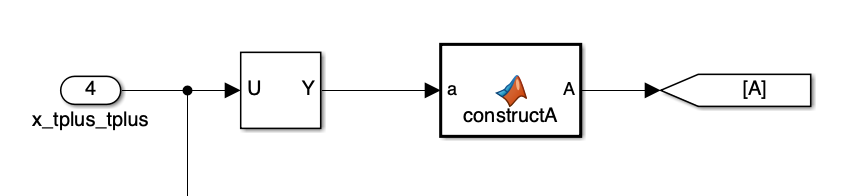
\includegraphics[width = 10cm]{Images/PS8/quat_update_2.png}
    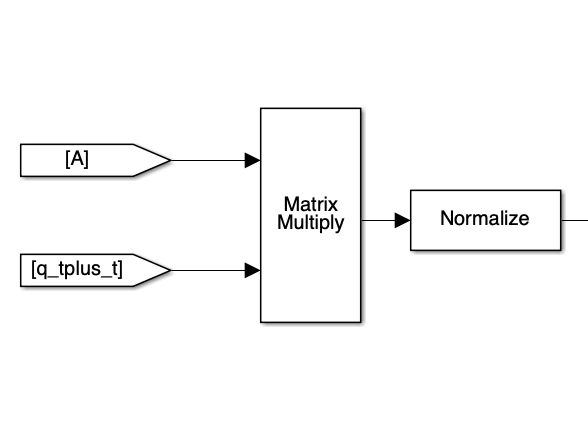
\includegraphics[width = 8cm]{Images/PS8/quat_update_1.png}
\end{figure}

\begin{figure}[H]
    \centering
    \captionsetup{ justification = centering }
    \begin{lstlisting}
function A = constructA(a)

ax = a(1);
ay = a(2);
az = a(3);

A = eye(4) + (1/2).*[0, -ax, -ay, -az;
                    ax, 0, az, -ay;
                    ay, -az, 0, ax;
                    az, ay, -ax, 0];
    \end{lstlisting}
    \caption{Simulink Model for Reset Step}
    \label{fig:quat_reset_step}
\end{figure}

Once this is computed, a rotation matrix can be obtained from the post-reset quaternion and used to recompute the measurement model. Now the residual can be computed using again Equation \ref{eq:meas_residual}.

For any plots and analysis regarding these residuals, the norm of this residual vector will be taken.

\subsection{Problem 7 - Produce plots showing true attitude estimation errors (estimate vs truth with statistics at steady state), formal or estimated attitude estimation errors (covariance from filter), pre- and post-fit residuals (with statistics at steady state), etc. Discuss the results, do they meet expectations? Is the true estimation error well described by the formal covariance? Are the measurements residuals consistent with the applied measurement errors? Hint: show estimation errors, do not overlap state estimate with reference truth.}

\begin{figure}[H]
    \centering
    \captionsetup{ justification = centering }
    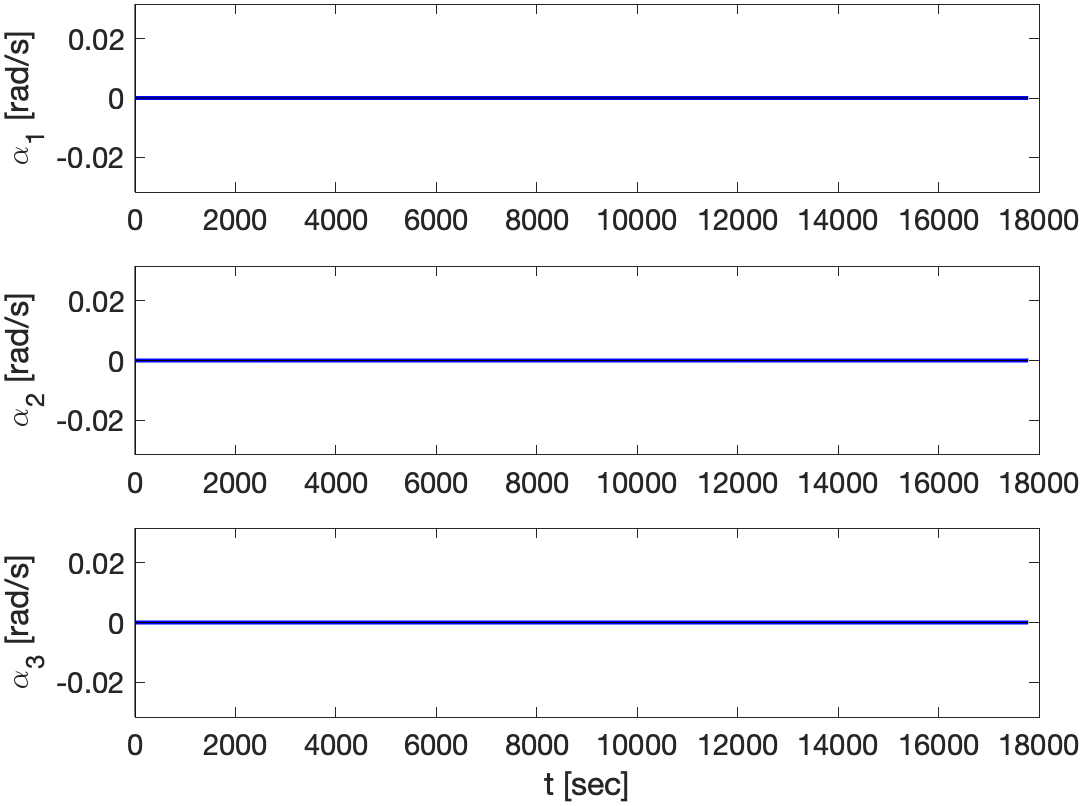
\includegraphics[width = 12cm]{Images/PS8/kalman_filter_meas_update_att_cov_bounds.png}
    \caption{Kalman Filter Covariance From Filter}
    \label{fig:kalman_att_cov}
\end{figure}

\begin{figure}[H]
    \centering
    \captionsetup{ justification = centering }
    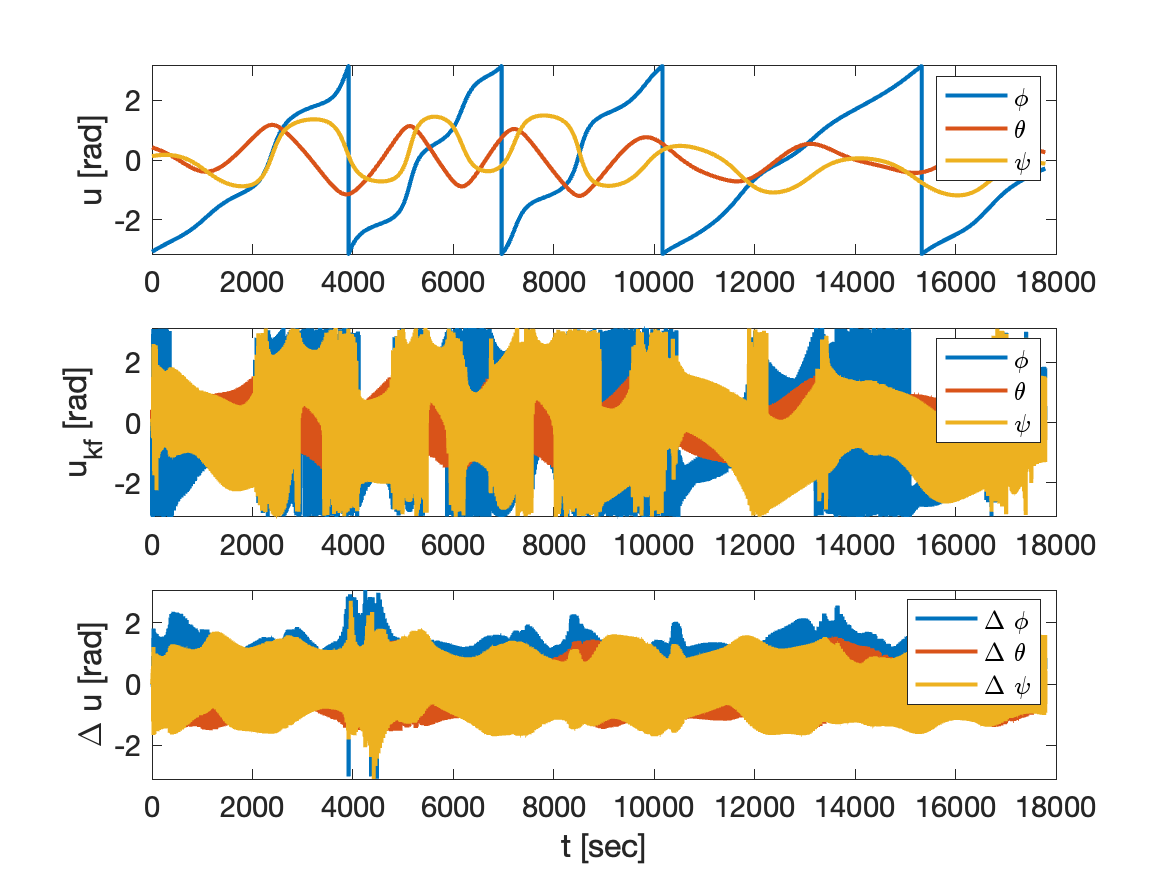
\includegraphics[width = 12cm]{Images/PS8/kalman_filter_meas_update_error_attitude.png}
    \caption{Kalman Filter Error for Attitude Measurements from Star Tracker and Magnetometer}
    \label{fig:kalman_error_attitude}
\end{figure}

\begin{figure}[H]
    \centering
    \captionsetup{ justification = centering }
    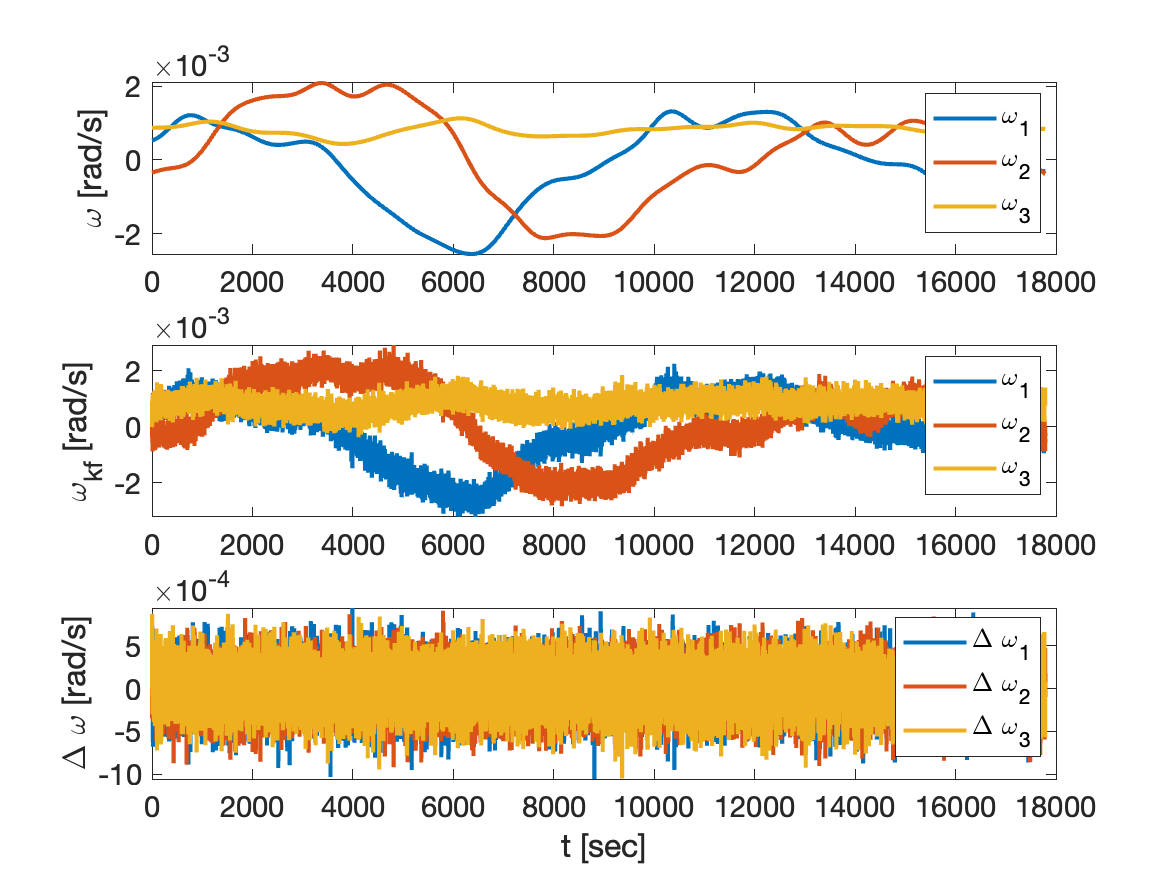
\includegraphics[width = 12cm]{Images/PS8/kalman_filter_meas_update_error_velocities.png}
    \caption{Kalman Filter Error for Velocity Measurements from Gyroscope}
    \label{fig:kalman_error_attitude}
\end{figure}

\begin{figure}[H]
    \centering
    \captionsetup{ justification = centering }
    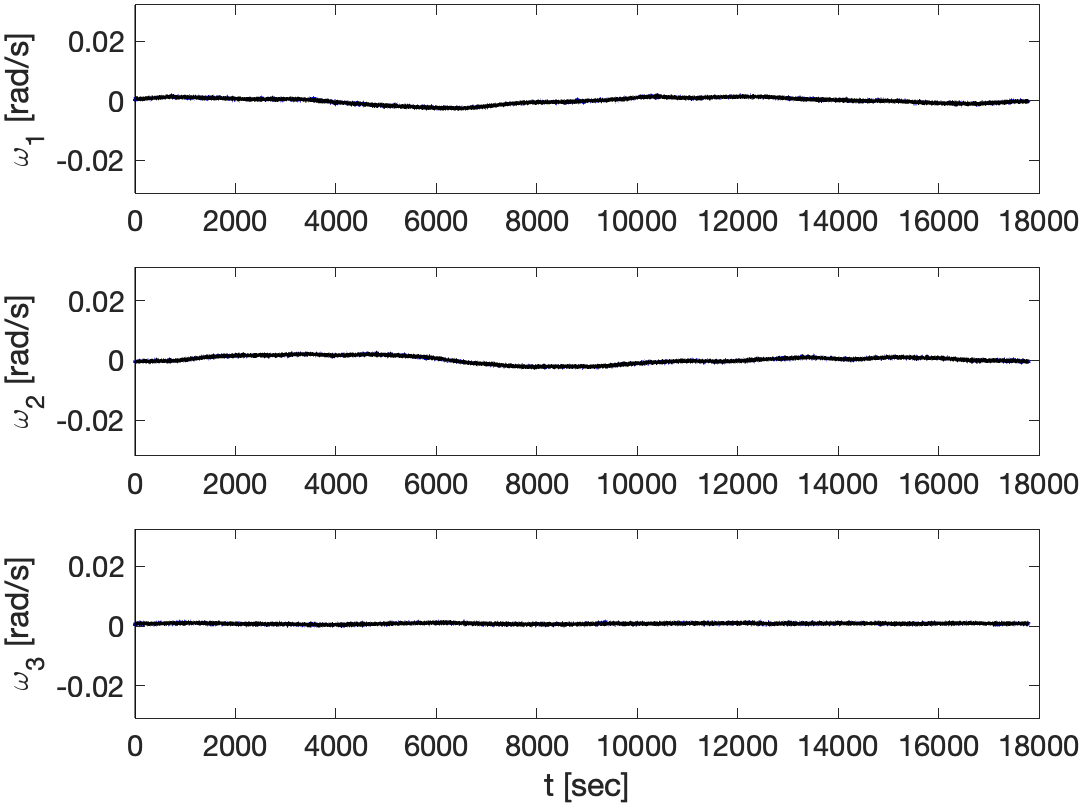
\includegraphics[width = 12cm]{Images/PS8/kalman_filter_meas_update_omega_cov_bounds.png}
    \caption{Kalman Filter $\omega$ Covariance From Filter}
    \label{fig:kalman_omega_cov}
\end{figure}

\begin{figure}[H]
    \centering
    \captionsetup{ justification = centering }
    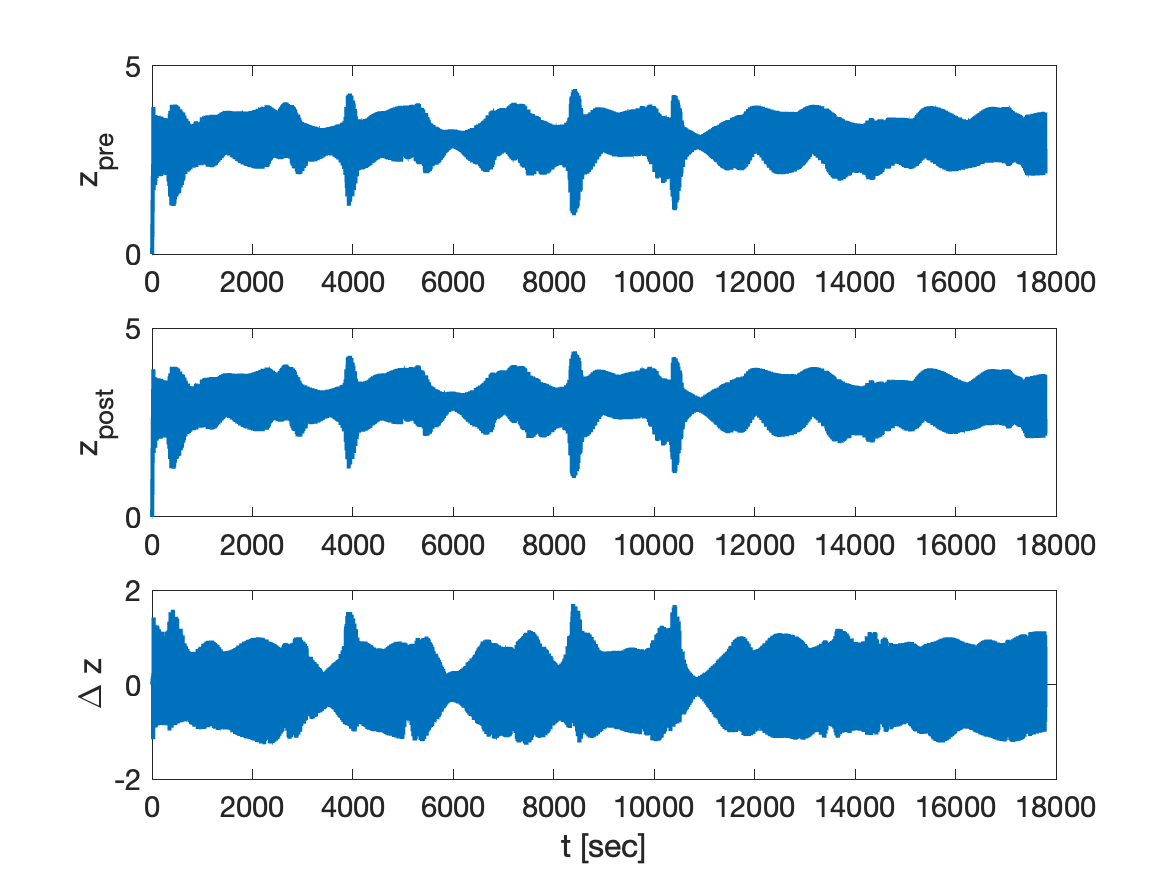
\includegraphics[width = 12cm]{Images/PS8/kalman_filter_meas_update_residual_comparison.png}
    \caption{Residual Comparison of Kalman Filter Update}
    \label{fig:kalman_residual}
\end{figure}

While these plots follow slightly similar trends to what would be expected, there is too much error between the true and predicted values for the filter to be working entirely correctly. This seems to indicate that an unresolved issue exists with our Kalman filter. While we haven't been able to find the source of this error, we currently believe that it likely lies within our star-tracker/magnetometer measurement model in the filter.

\subsection{Problem 8 - Start thinking/planning possible upgrades for the final project deliverable. Upgrades can go in several directions tailored to your project needs. For example, define different modes for attitude estimation using different sensors and algorithms based on your concept of operations. What would it take to implement a UKF instead of an EKF? Can you improve your dynamics and measurement models? Can you use measurements that are more representative of what your sensors are going to actually provide you?}

In the previous homework, the sensors were only modelled to the depth of assuming that they output unit vector measurement of the star location or gravitational field that
include errors from a constant bias and Gaussian noise. However, it would be much more accurate to assume that they output voltage values that then need to be converted to meaningful measurements. Because of this, a lower level hardware model of the attitude sensors would be beneficial to implement as that would align with the scope of what was needed for the Aqua satellite. Another option for the final project would be to implement a mode of operation where instead of pointing towards the Earth, the satellite would communicate with another satellite in the same orbit. The Aqua satellite was one of several science missions launched by NASA into similar low Earth orbits. These satellites formed a train over the several years that they were all launched in. To the best of our knowledge, the satellites in this train were not able to communicate with each other due to the big gaps in technology between their launches. However, if they were, they could use those connections to help with down linking data and other tasks. Because of this, it would be interesting to define another mode of operation where the satellite would point to another artifical satellite in its orbit.